\chapter{Material und Methoden}
\label{ch:methodik}

\section{Versuchsaufbau}
Abbildung~\ref{fig:pendel} zeigt eine eigens erstellte schematische
Darstellung eines Fadenpendels. In einer echten Arbeit gehören hier
Fotos oder Skizzen des \emph{tatsächlich verwendeten} Aufbaus hinein.

\begin{figure}[htbp]
  \centering
  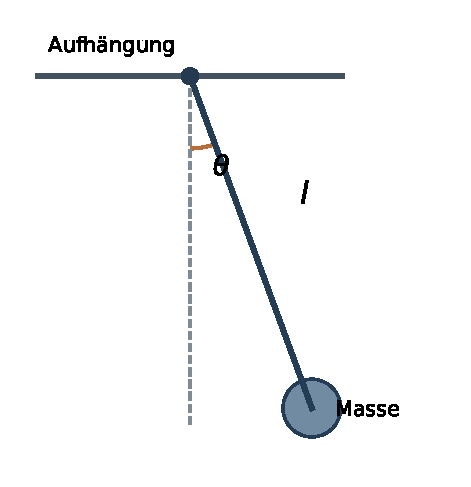
\includegraphics[width=.6\linewidth]{abbildungen/pendel-schema.pdf}
  \caption{Schematisches Fadenpendel (eigene Illustration für die Vorlage)}
  \label{fig:pendel}
\end{figure}

\section{Messverfahren und Dokumentation}
\textbf{Beispiel für eine mögliche Planung (nicht durchgeführt):}
Die Länge wird zwischen Aufhängepunkt und Schwerpunkt der Masse
bestimmt. Für mehrere Längen werden jeweils zehn Perioden zeitlich
erfasst. Die Zeit pro Periode ergibt sich aus der Division der
Gesamtmesszeit durch zehn. Jede Einstellung wird mehrfach wiederholt.

\section{Auswertung und Unsicherheiten}
Bei einer echten Messung müssen Gerätetypen, Kalibrierung,
Messwiederholungen und Unsicherheiten nachvollziehbar angegeben werden.
Eine mögliche Auswertungsgröße wäre \(T^2\), die nach
Gleichung~\eqref{eq:pendel} linear mit \(l\) zusammenhängt.
% WICHTIG: echte Rohdaten, Messprotokolle und Auswertungscode aufbewahren.
